\chapter{Multiple Action Policy Gradients}\label{chapter:map_algo}
In this section, we describe the Multiple Action Policy Gradient algorithm and give a simple proof why MAPG converges to a better policy. Further, we propose the MAPG version of Deep Deterministic Policy Gradient (DDPG).


\section{Multiple Action Prediction}
Multiple action prediction idea is inspired by multiple hypothesis prediction \cite{rupprecht2017iccv} for supervised learning. The basic idea behind multiple action prediction is to propose $M$ actions at each time step for a reinforcement learning agent. The agent uniformly samples one action out of these $M$ proposed actions. This formulation makes the policy stochastic and is useful in continuous reinforcement learning tasks. We call the class of policy gradient algorithms using this formulation as Multiple Action Policy Gradients (MAPG). Although, multiple action prediction is general enough and can be used with any existing reinforcement learning algorithm, in this work we only consider policy gradient methods with multiple action prediction.

\begin{figure}[htb]
    \centering
    \frame{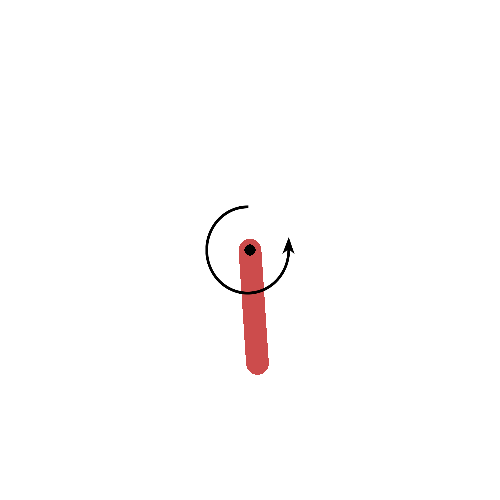
\includegraphics[width=.5\linewidth]{figures/04/inv_pendulum.png}}
    \caption{Screenshot of \env{Pendulum} environment. In this position the pendulum has two equally good actions, it can either move left or right to reach the target vertically upward position.}
    \label{fig:04_pendulum}
\end{figure}


MAPG is based on the intuition that the resulting policy is stochastic which leads to a better exploration of the entire solution space as well as a final solution of potentially higher quality. It can also help in eliminating the external exploration mechanisms required during training e.g. Ornstein-Uhlenbeck process noise \cite{ounoise}, parameter noise \cite{paramnoise} or differential entropy of the normal distribution.

A simple example of inverted pendulum cart balancing task where MAPG is useful is illustrated in Figure \ref{fig:04_pendulum}. In this task, the goal is to balance the pendulum upside down. The agent can control the movement by moving the cart to left or right. The pendulum is currently hanging vertically and has two equally promising actions to reach final goal: either moving left or right. A deterministic agent chooses a single action for every state, this breaks the inherent symmetry of the task. Other distribution parameter estimation methods (e.g. A3C, NAF) might work better than deterministic policies in this case as there are only two good options, but in cases when there are more than two good actions to select, this will not be optimal. MAPG allows the agent to suggest multiple actions, which enables it to resolve cases like this easily. 

% \subsection{Background}

\section{Optimal Policy for MAPG} \label{03:mapg_proof}
MAPG produces multiple actions which can be viewed as $M$ different policies. Here, we show that MAPG learns an optimal policy and all learned $M$ policies are equally good.
We investigate a typical reinforcement learning setup introduced in Chapter \ref{chapter:background}.

We consider the Bellman equation for Q-value function from Eqn. \ref{eq:bellman_q}. Methods such as (D)DPG use a deterministic policy where each state is deterministically mapped to an action using a function $\pi: \mathcal{S}\rightarrow\mathcal{A}$ which simplifies Eqn. \ref{eq:bellman_q} to

\begin{equation}\label{eq:deterministicbellman}
Q_\pi(s_t,a_t) = \mathbb{E}_{r_t,s_{t+1}\sim E}[r(s_t,a_t) + \gamma Q_\pi(s_{t+1},\pi(s_{t+1}))].
\end{equation}

The $Q$ value of an action is approximated by a critic network which estimates $Q_\pi(s_t,a_t)$ for the action chosen by the actor network.

The key idea behind predicting multiple actions is that it is possible to learn a stochastic policy as long as the inner expectation remains tractable. Multiple action prediction achieves this by predicting a fixed number $M$ of actions $\rho: \mathcal{S}\rightarrow\mathcal{A}^M$ and uniformly sampling from them. The expected value is then the mean over all $M$ state-action pairs. The state-action value can then be defined as
\begin{align}
 Q_\rho(s_t,a_t) = & \mathbb{E}_{r_t,s_{t+1}\sim E} \nonumber \\&  \left[r(s_t,a_t) + \gamma \frac{1}{M} \sum_{m=1}^M Q_\rho(s_{t+1},\rho_m(s_{t+1}))\right].
 \label{eq:mapbellman}
\end{align}

This is beneficial since we not only enable the agent to employ a stochastic policy when necessary, but we also approximate the action distribution of the policy with multiple samples instead of one. 

There exists an intuitive proof that the outer expectation in Eqn. \ref{eq:mapbellman} will be maximal if and only if the inner $Q_\rho$ are all equal. The idea is based on the following argument: let us assume $\rho$ as an optimal policy maximizing Eqn. \ref{03:eq_pg}. Further, one of the $M$ actions $\rho_j(s_{t+1})$  for a state $s_{t+1}$ has a lower expected return than another action $k$,
\begin{equation}\label{key}
Q_\rho(s_{t+1},\rho_j(s_{t+1})) < Q_\rho(s_{t+1},\rho_k(s_{t+1})).
\end{equation} 
Then there exists a policy $\rho^*$ that would score higher than $\rho$ that is exactly the same as $\rho$ except that it predicts action $k$ instead of $j$: $\rho^*_j(s_{t+1}) := \rho_k(s_{t+1})$. However, this contradicts the assumption that we had learned an optimal policy beforehand. Thus in an optimal policy all $M$ action proposals will have the same expected return. 
More informal, this can also be seen as a derivation from the training procedure. If we always select a random action from the $M$ proposals, they should all be equally good since the actor cannot decide which action will be executed.

From the proof, it directly follows that it is possible - and sometimes necessary - that all proposed actions are identical. This is the case in situations where there is just one single right action to take. When the action proposals do not collapse into one, there are two possibilities: either it does not matter what action is currently performed, or all proposed actions lead to the desired outcome. 

Naturally, the set of stochastic policies includes all deterministic policies, since a deterministic policy is a stochastic policy with a single action having probability density equal to one. This means that in theory, we expect the multiple action version of a deterministic algorithm to perform better or equally well since it could always learn a deterministic policy by predicting $M$ identical actions for every state.

In the experimental section, we will investigate if the predicted value for each of the $M$ actions is indeed similar during an episode. 

\newpage
\section{DDPG with MAPG}
Here we modify deep deterministic policy gradient (DDPG) algorithm to use MAPG. DDPG is based on actor-critic architecture, where actor network produces a deterministic policy $\pi(s)$ for a state $s$. To make DDPG use MAPG, we modify the last layer of actor network and output $M$ action vectors. During training of the algorithm, one out of $M$ action vectors is uniformly sampled and index $j$ of the chosen action vector is saved along with transition $(s_t, a^j_t, s_{t+1}, r_t) $. Now, during optimization of the actor network, the policy gradient is only propagated through the branch connected by $j$ at the last layer. Over time each branch in the last layer will be selected equally often, thus every branch will be updated and learned during training. 


% This training process is illustrated in Figure \ref{fig:05_mapg}.
Algorithm \ref{alg:ddpgmap} outlines the MAPG algorithm in detail. 


\newpage

\begin{algorithm}[h]
  \caption{DDPG with MAPG algorithm}
  \label{alg:ddpgmap}
\begin{algorithmic}
  \STATE Modify actor network $\pi(s|\theta_\pi)$ to output $M$ actions,  $A_t = \{\rho_1(s_t), \ldots, \rho_M(s_t) \} $.
  \STATE Randomly initialize actor $\pi(s|\theta_\pi)$ and critic $Q(s, a|\theta_Q)$ network weights.
  \STATE Initialize target actor $\pi'$ and critic $Q'$ networks, $\theta_\pi' \gets \theta_\pi$ and $\theta_Q' \gets \theta_Q$.  
  \FOR{$\text{episode}=1$ {\bfseries to} $N$}
  \STATE Initialize random process $\mathcal{N}$ for exploration.
  \STATE Receive initial observation/state $s_1$.
  \FOR{$t=1$ {\bfseries to} $T$}
  \STATE Predict $M$ action proposals $A_t = \{\rho_1(s_t), \ldots, \rho_M(s_t) \} = \pi'(s_t|\theta_\pi)$.
  \STATE Uniformly sample an action $j$ from $A_t$: $a^j_t = \rho_j(s_t) + \mathcal{N}_t$.
  \STATE Execute action $a^j_t$ and observe reward $r_t$ and state $s_{t+1}$.
  \STATE Store transition $(s_t, a^j_t, r_t, s_{t+1})$ to replay buffer $R$.
  \STATE Sample a random batch of size $B$ from $R$.
  \STATE Set $y_i = r_i + Q'(s_{i+1}, \pi'(s_{i+1}|\theta_\pi')|\theta_Q')$.
  \STATE Update critic by minimizing the loss, 
  \STATE \hspace{2em} $L = \frac{1}{B} \sum_{i} (y_i - Q(s_i, a^j_i|\theta_Q))^2$    

  \STATE Update all actor weights connected to $a^j_t$. %, i.e. $\theta_\pi - \theta_\pi^{\{1 \dots M\}}+ \theta_\pi^j$.

   \STATE \hspace{2em} $\nabla_{\theta^\pi} J \approx \frac{1}{B} \sum_{i} \nabla_{a^j_i}Q(s, a| \theta^Q)|_{s=s_i, a=a^j_i} \nabla_{\theta_\pi - \theta_\pi^{\{1 \dots M\}}+ \theta_\pi^j} \pi(s|\theta^\pi)|_{s_i}$
   
  \STATE Update the target networks: 
  \STATE \hspace{2em} $\theta_\pi' \gets \tau\theta_\pi' + (1-\tau)\theta_\pi$
  \STATE \hspace{2em} $\theta_Q' \gets \tau\theta_Q' + (1-\tau)\theta_Q$
  \ENDFOR
  \ENDFOR
\end{algorithmic}
\end{algorithm}

